\documentclass[11pt]{article}
\usepackage[margin=2.6cm]{geometry}
\usepackage{amsmath,amssymb}
\usepackage{graphicx}
\usepackage[colorlinks=true,linkcolor=blue,citecolor=blue,urlcolor=blue]{hyperref}
\usepackage{booktabs}
\usepackage{xeCJK}
\setCJKmainfont{Hiragino Mincho ProN}
\setCJKsansfont{Hiragino Sans}
% AUTO-GENERATED by scripts/make_paper_numbers.py — DO NOT EDIT
% source commit: 3d8fdbb
\newcommand{\NmAndEta}{11.53}
\newcommand{\NmAndMf}{9.5\times10^{-16}}
\newcommand{\NmAndMfArr}{9.1\times10^{-31}}
\newcommand{\NmSgrEta}{6.947}
\newcommand{\NmSgrMf}{8.9\times10^{-10}}
\newcommand{\NmSgrMfArr}{7.9\times10^{-19}}
\newcommand{\NmTraEta}{0.740}
\newcommand{\NmTraMf}{0.108}
\newcommand{\NmProxEta}{0.0849}
\newcommand{\NmProxMf}{0.775}
\newcommand{\NmProxEtaRT}{0.169}
\newcommand{\NmTraEtaRT}{1.260}
\newcommand{\NmSgrEtaRT}{7.640}
\newcommand{\NmAndEtaRT}{12.22}
\newcommand{\NmTflQ}{2.58\times10^{3}}
\newcommand{\NmTeffQ}{1.22}
\newcommand{\NmTceilQ}{0.824}
\newcommand{\NmTflXII}{5.98\times10^{18}}
\newcommand{\NmTeffXII}{31.1}
\newcommand{\NmTceilXII}{30.4}
\newcommand{\NmXstar}{0.54}
\newcommand{\NmLamstar}{0.13}
\newcommand{\NmEtaFb}{0.366}
\newcommand{\NmMassMsunKm}{0.102}
\newcommand{\NmMassKgKm}{2.02\times10^{29}}
\newcommand{\NmLpeakW}{3.1\times10^{51}}
\newcommand{\NmLpeakLsun}{8.1\times10^{24}}
\newcommand{\NmBurnMuS}{17.6}
\newcommand{\NmRadEtaQ}{51.3}
\newcommand{\NmSeatXII}{2.6\times10^{10}}
\newcommand{\NmGRowsP}{306}
\newcommand{\NmSigRows}{567}
\newcommand{\NmMapMission}{5.0\times10^{-15}}
\newcommand{\NmMapRide}{1.06\times10^{-6}}
\newcommand{\NmFlashPeak}{1.48\times10^{4}}
\newcommand{\NmFlashExp}{72}
\newcommand{\NmFlashDecay}{5\times10^{-6}}
\newcommand{\NmFlashPs}{15}
\newcommand{\NmWtCommit}{1e9e3db}
\newcommand{\NmRepoCommit}{3d8fdbb}


\title{正エネルギーワープシェルの恒星間飛行プロファイルと観測署名}
\author{前田 幸枝(Yukie Maeda)\\ \small Independent Researcher, Tokyo\\
\small ORCID: 0009-0005-3401-9230}
\date{2026(英語正本の忠実訳。数値・表・図は英語版と同一の生成物を参照する)}

\begin{document}
\maketitle

\begin{abstract}
正エネルギー物質のみで構成され加速するワープシェルの存在は、最近確立された。
Le の放射運動量ワープシェル~\cite{le-steering}は、閉形式のコスト法則と
加速・コンパクト度フロンティアの下で、光子ロケットの反作用により操舵する。
その構成に含まれていないのは飛行計画である。系統的検索(被引用スキャン、
論文全文の精読、著者の公開再現コードの検査)は、シェルの許容性制約の下での
恒星間航路計算が公表されていないことを確認した。本論文はそのカタログを計算
する。厳密な天井、数値的にマップされたフロンティア帯、暫定的な厳密床という
拘束の全構成の下で、プロキシマ・ケンタウリ、TRAPPIST-1、いて座A*、M31 への
燃料・時間表を得る。乗員寿命の等高線($\tau = 50$ 年)は M31 フライバイに
巡航ラピディティ $\eta = \NmAndEta$ を要求し、質量比は
$m_f/m_0 = \NmAndMf$ である。時間最適プロファイルは動くフロンティアに騎乗し、
操作的拘束はコンパクト度 $x^* \approx \NmXstar$ で薄殻フロンティアから厚壁
実現可能性へ切り替わる。同じ積分が観測署名を与える。飽和加速中のシェルは
目的地方向に厳密に暗く、到着は $\delta^4 = e^{4\eta}$ で増幅され到着時間で
圧縮された減速フラッシュとして告げられる。その減衰は一般則
$F \propto e^{7\eta - 3\Delta\eta_{\rm tot}}$(M31 到着では
$e^{7\eta-\NmFlashExp}$、ピコ秒級の時間構造)に従い、その間 Damour 双極子の
上で重力波は無音である。すべての数値は認証済みカタログから機械注入される
(機動層 $\NmGRowsP$ 行、署名層 $\NmSigRows$ 行、二経路照合・欠番ゼロ)。
検証記録には著者コードとの相互検証 6 件と再現性ギャップ 1 件が含まれ、
後者は見出されたとおりに記す。
\end{abstract}

\section{序論}\label{sec:intro}

ワープドライブの文献は、交わらない二つの系譜に分かれてきた。一方はシェルが
何でありうるかを証明する系譜である。Alcubierre の計量~\cite{alcubierre}は
負エネルギーを要求し、Santiago, Schuster, Visser の no-go~\cite{ssv}、
Pfenning と Ford の量子不等式~\cite{pfenning}、Lobo と Visser の固有値
解析~\cite{lobo}は、この欠陥が計量先行型の設計に一般的であることを確立した。
Lentz の正エネルギーソリトン~\cite{lentz}は精査に耐えなかった。零渦度
ソリトンの Euler 系エネルギー密度は各スライスで積分するとゼロになり~\cite{ssv}、
直接の Euler 系計算が負の領域を示した~\cite{celmaster}。ソース先行型の構成は、
静的または定速の、真に正エネルギーのシェルを生んだ。Bobrick と Martire の
分類~\cite{bobrick}、および Warp Factory~\cite{helmerich}で数値的に検証された
Fuchs らの定速シェル~\cite{fuchs}である。Le は加速の欠落を閉じた。放射運動量
ワープシェル~\cite{le-steering}は、平坦な乗客キャビティを厳密な Kinnersley
光子ロケット~\cite{kinnersley}に接合された時間的シェルで包み、バルクと
シェルの双方で優勢エネルギー条件を満たし、閉形式の制御則 $-\dot m \geq
3m|a|$ と Tsiolkovsky 予算 $m_f/m_0 = e^{-3\Delta\eta}$ の下で操舵する。

他方は点質量がどこへ飛べるかを計算する系譜である。F\"uzfa~\cite{fuzfa2019}は
裸の Kinnersley ロケットによる恒星間航行をモデル化し、プロキシマ行きの軌道、
エネルギーコスト、光行差、Doppler 偏移を導出し、続報でレーザー推進帆へ
天体力学を拡張した~\cite{fuzfa2020}。これらの計算には乗客キャビティも、
接合されたシェルも、シェルを物理的たらしめる許容性制約も含まれていない。

系統的検索、すなわち arXiv:2606.22531 の被引用スキャン(Semantic Scholar
および INSPIRE-HEP、2026-08-08、被引用ゼロ)、v3 の全文精読、コミット
\NmWtCommit{} に固定した著者の公開再現コード~\cite{worldtube}の検査は、
シェルの許容性制約の下での恒星間飛行プロファイルの計算が公表されていない
ことを確認した。本論文はその計算を実行し、観測可能な帰結を導出する。

本論文の貢献は四点である。第一に、許容性制約つき機動カタログである。
行き先に依存しないラピディティ階段、四つの行き先に対するミッション表と
乗員寿命等高線、そして理想光子ロケットに対する乗客輸送の「座席の値段」を
与える。第二に、三層拘束系での時間最適プロファイルであり、
$x^* \approx \NmXstar$ の拘束レジーム交差を含む(我々の知る限り未定量化。
第\ref{sec:results}節C)。第三に、全プロファイルを観測者系光度曲線に写す
署名カタログであり、飽和加速の厳密な前方ヌル、閉形式減衰則に従う減速
フラッシュ、重力波静寂判別子を与える。第四に、検証方法論(認証テスト、
二経路照合、権威ラベル、AI 作業に対する人間の決定ゲート)であり、その記録は
著者コードとの相互検証 6 件と再現性ギャップ 1 件を含む
(第\ref{sec:methods}節に事実として記す)。

\section{枠組み}\label{sec:framework}

文献~\cite{le-steering}の枠組みを公表されたとおりに用い、再導出は行わない。
外部は外向きヌルダストを源とする Kinnersley--Robinson--Trautman 光子ロケット
であり、静止系の排気パターンは厳密な双極子 $4\pi n^2(\vartheta) = -\dot m -
3ma\cos\vartheta$(文献~\cite{le-steering}の式(13))である。ここで
$\vartheta$ は各遅延カットの瞬間静止系で固有加速軸から測る。バルクの
エネルギー条件は $n^2 \geq 0$ に帰着し、その前方極での束縛が制御則
$-\dot m \geq 3m|a|$(式(14))と予算 $m_f/m_0 = e^{-3\int|a|\,du}$
(式(15))を与える。静的アンカーは $x = 2m/R < 24/25$(式(25))で表面優勢
エネルギー条件を満たし、外部の正則な葉層は加速を運動学的天井 $\lambda = aR
< \tfrac{1}{2}(1-x)$(式(40))で抑え、有限厚(接線圧)壁としての実現可能性は
後方極実効コンパクト度に $x + 2\lambda < 4/5$(文献~\cite{le-steering}の
第10節)を要求する。

公表するすべての数値は、厳密閉形式、数値マップ、発見法を区別する原論文の
流儀に従い、権威ラベルを相続する。[R] は厳密閉形式、[N] は公表数値への依拠
(サンプル域内でのみ使用)、[H] は発見法(表示のみ、拘束には不使用)を表す。
操作的拘束系は三層である(表~\ref{tab:tiers})。厳密な天井
$\min\{\tfrac12(1-x), \tfrac12(\tfrac45 - x)\}$ [R]、実効帯
$\underline{g}(x)$ [N](文献~\cite{le-steering}の観測者ロバストな
フロンティアスキャン、$x \in [0.1, 0.7]$)、そして床 $c_{\rm cons}(x)$
である。床は論文の厳密下界鎖の保守的独立評価であり、第\ref{sec:methods}節に
記す理由により暫定ラベルで運用する。騎乗プロファイルはすべて天井を
ハードクランプとして併課する。

\begin{table}[t]
\centering
\caption{$\lambda = aR$ に対する三層拘束系。}
\label{tab:tiers}
% AUTO-GENERATED by scripts/make_paper_numbers.py — DO NOT EDIT
\begin{tabular}{llll}
\hline
Tier & Bound on $\lambda=aR$ & Authority & Domain \\
\hline
Ceiling & $\min\{\tfrac12(1-x),\,\tfrac12(\tfrac45-x)\}$ & [R] (unattainable upper limit) & $x\in(0,4/5)$ \\
Effective & $\underline{g}(x)$, linear interpolation & [N] (no extrapolation) & $x\in[0.1,0.7]$ \\
Floor & $c_{\rm cons}(x)$ & [R(A3)/provisional] & $x\in(0,4/5)$ \\
\hline
\end{tabular}

\end{table}

\section{方法}\label{sec:methods}

\subsection{検証プロトコル}

計算は単一のコードではなく、検証されたパイプラインとして組織した。式は
原論文から転記した式台帳を通じて入り(全体で v3 基準。v2 から v3 への式番号
変更は台帳に対応表がある)、実装された式はどれも、論文に印字された数値を
再現する認証テストに合格するまで下流で使用できない。認証スイートは
Tsiolkovsky 予算と表面エネルギー条件窓から署名層の観測者系パターン正規化
まで、18 の関門(C1--C18)を含む。主要量は二つの独立経路(閉形式と独立数値)
で計算し、不一致は黙って許容を広げる対象ではなく停止条件である。カタログは
機動層 \NmGRowsP{} 行、署名層 \NmSigRows{} 行の照合済み行を持ち、欠番はない。

経路一致の許容は二種である。閉形式が利用可能な行は $10^{-8}$ を満たし、
ミッション級の遅延時間写像は $\NmMapMission$ で一致する。フロンティア騎乗
プロファイルでは遅延時間写像の二実装が、文書化されたクラス許容
$2\times10^{-6}$ に対し $\NmMapRide$ で一致する。保存された騎乗グリッドが
補間を情報制限する(区分線形 $\underline{g}$ の折れ点がグリッド区間の内部に
落ち、$x_0=0.7$ の序盤では $\lambda$ の勾配が急である)ためであり、残差は
実装ではなく消費データの性質を反映する。このクラス許容自体が、許容の変更は
人間の承認事項であるという運用規則の下、人間の決定ゲート(2026-08-09)で
裁定された。

本論文のすべての数値主張は、表の項目と図のキャプションを含めて、認証済み
カタログから生成マクロ層を通じて機械注入される。マニフェストが注入値ごとに
ソースフィールドと表示変換を記録し、認証テストが原稿の裸数値を走査し
マニフェストを再計算する。

\subsection{AI の関与}

すべての計算、実装、原稿起草は、人間ゲート付きプロトコルの下で Claude
(Fable 5, Anthropic)が行った。各フェーズの成果物は明示的な人間の決定
ゲートでレビューと承認を受け、すべての数値主張は認証済みカタログから機械
注入され、許容の変更自体が人間ゲートの裁定事項であった。

\subsection{著者コードとの相互検証と一件のギャップ}

著者の公開再現コード~\cite{worldtube}をコミット \NmWtCommit{} に固定し、
六件の一致を得た。フロンティアの数値ピン $\underline{g}(x)$ は我々の転記と
完全に一致する。軸マージンの式(文献~\cite{le-steering}の式(42))は逐語一致
する。凍結軸閾値と天井の最悪比($x \approx 0.631$ での $0.9931$)は我々の
転記のみから独立に再現される。閉形式推定の精度主張はその適用域で確認される。
凍結マージン係数は記号的に一致する。そしてコードは v2 の分岐スカラーが v3 で
除去されたことを明文で述べており、我々が独立に同定しハーネスで隔離した構造的
撤回を著者側から確認する。

一つの量が検証に抵抗した。式(73)の床の評価値は、論文本文と公開コードから
独立に再現できなかった。必要な三つの上限量は両方の資料で手続き的に記述される
が、どちらにも閉形式では与えられていない。そこで保守的な独立床を構成し、
暫定ラベルを付した。我々の $c_{\rm cons}(x)$ は五つのサンプル点すべてで印字値
より厳密に下にあり、印字された束縛枝構造を再現する。その鎖のすべての段階は
印字された閉形式か、文書化された読みの下での証明可能な過大評価であるから、
その読みの範囲では真の下界である。この不一致は誤りの主張ではなく再現性の
記述として記録し、本論文のすべての成果物の床 tier は暫定ラベルを保持する。

\section{結果}\label{sec:results}

\subsection{ラピディティ階段と座席の値段}

燃料は行き先に依存しない。$m_f/m_0 = e^{-3\Delta\eta}$ は積分ラピディティ
のみに依存するから、最初のカタログ表(表~\ref{tab:ladder})には距離の列が
ない。news 静寂な排気に必須の双極子の広がりにより、乗客シェルは理想的な
コリメート光子ロケットが $e^{\eta}$ を払うところで $e^{3\eta}$ を払う。
両者の比、すなわち座席の値段は $e^{2\eta}$ である。実働バーンのラピディティ
$\eta = 0.24$ でシェルは静止質量の $\NmRadEtaQ\%$ を放射し(原論文の実働
機動と一致。我々のスイートはこれを認証 C4 として再現する)、座席の値段は
$1.6$ に留まる。$\eta = 12$ では座席の値段は $\NmSeatXII$ に達する。

\begin{table}[t]
\centering
\caption{ラピディティ階段(行き先非依存、全行 [R])。$1-\beta$ 列は
$\beta$ の表示桁が飽和する光速接近を分解する。座席の値段は理想コリメート
光子ロケットに対する初期質量比である。}
\label{tab:ladder}
% AUTO-GENERATED by scripts/make_paper_numbers.py — DO NOT EDIT
\begin{tabular}{rrrrrr}
\hline
$\eta$ & $\beta$ & $1-\beta$ & $m_f/m_0$ & radiated & seat price $e^{2\eta}$ \\
\hline
0.24 & 0.2355 & $7.6\times10^{-1}$ & $4.9\times10^{-1}$ & 51.3\% & $1.6\times10^{0}$ \\
1 & 0.7616 & $2.4\times10^{-1}$ & $5.0\times10^{-2}$ & 95.0\% & $7.4\times10^{0}$ \\
3 & 0.9951 & $4.9\times10^{-3}$ & $1.2\times10^{-4}$ & 100.0\% & $4.0\times10^{2}$ \\
5 & 0.9999 & $9.1\times10^{-5}$ & $3.1\times10^{-7}$ & 100.0\% & $2.2\times10^{4}$ \\
8 & 1.0000 & $2.3\times10^{-7}$ & $3.8\times10^{-11}$ & 100.0\% & $8.9\times10^{6}$ \\
12 & 1.0000 & $7.6\times10^{-11}$ & $2.3\times10^{-16}$ & 100.0\% & $2.6\times10^{10}$ \\
\hline
\end{tabular}

\end{table}

\subsection{ミッション表と乗員寿命等高線}

ミッション運動学(双曲バーンと一定ラピディティの巡航)は階段を四つの行き先
(プロキシマ・ケンタウリ、TRAPPIST-1、いて座A*、M31。カタログ距離は
データ公開物に典拠つきで固定)の時刻表へ変換する。キロメートル級シェルの
バーン時間はマイクロ秒であるから、ミッション時間は巡航支配であり、船内
固有時間は $\tau \approx D/\sinh\eta$ である。表~\ref{tab:contour}は乗員
寿命等高線 $\tau = 50$ 年を報告する。プロキシマのフライバイは
$\eta = \NmProxEta$、質量比 $\NmProxMf$ で足りる。いて座A*は
$\eta = \NmSgrEta$、質量比 $\NmSgrMf$。M31 のフライバイは
$\eta = \NmAndEta$、$m_f/m_0 = \NmAndMf$ を要する。到着(目的地系への減速)
は指数を倍にし、往復は四倍にする。M31 到着は $\NmAndMfArr$ を要するが、
予算は全経路で正エネルギーであるから、これはミッションを禁じるのではなく
値付けする。往復では寿命条件が往復全体の固有時間に適用されるため、
表~\ref{tab:contour}の往復列はそれ自身の巡航ラピディティ
$\eta_{\rm RT} = {\rm arcsinh}(2D/\tau)$(M31 では
$\eta_{\rm RT} = \NmAndEtaRT$)で評価し、その燃料列は
$\Delta\eta_{\rm tot} = 4\eta_{\rm RT}$ を用いる。
図~\ref{fig:contour}は階段全域の等高線を示す。

\begin{table}[t]
\centering
\caption{乗員寿命等高線($\tau = 50$ 年、船内固有時間。バーンは厳密に算入、
巡航支配)。フライバイと到着の列は $\eta_{50} = {\rm arcsinh}(D/\tau)$ を
共有し、往復列はそれ自身の $\eta_{\rm RT} = {\rm arcsinh}(2D/\tau)$、
すなわち往復全体の固有時間が等高線に達するラピディティで評価する。燃料列は
$m_f/m_0 = e^{-3\Delta\eta_{\rm tot}}$、$\Delta\eta_{\rm tot} = \eta_{50},
2\eta_{50}, 4\eta_{\rm RT}$ である。}
\label{tab:contour}
% AUTO-GENERATED by scripts/make_paper_numbers.py — DO NOT EDIT
\begin{tabular}{lrrrrrr}
\hline
Destination & $D$ [ly] & $\eta_{50}$ & $\eta_{\rm RT}$ & $m_f/m_0$ (flyby) & (arrive) & (round trip) \\
\hline
Proxima Centauri & 4.25 & 0.085 & 0.169 & 7.8e-01 & 6.0e-01 & 1.3e-01 \\
TRAPPIST-1 & 40.5 & 0.740 & 1.260 & 1.1e-01 & 1.2e-02 & 2.7e-07 \\
Sgr A* & $2.6\times10^{4}$ & 6.947 & 7.640 & 8.9e-10 & 7.9e-19 & 1.5e-40 \\
M31 (Andromeda) & $2.54\times10^{6}$ & 11.529 & 12.222 & 9.5e-16 & 9.1e-31 & 2.0e-64 \\
\hline
\end{tabular}

\end{table}

\begin{figure}[t]
\centering
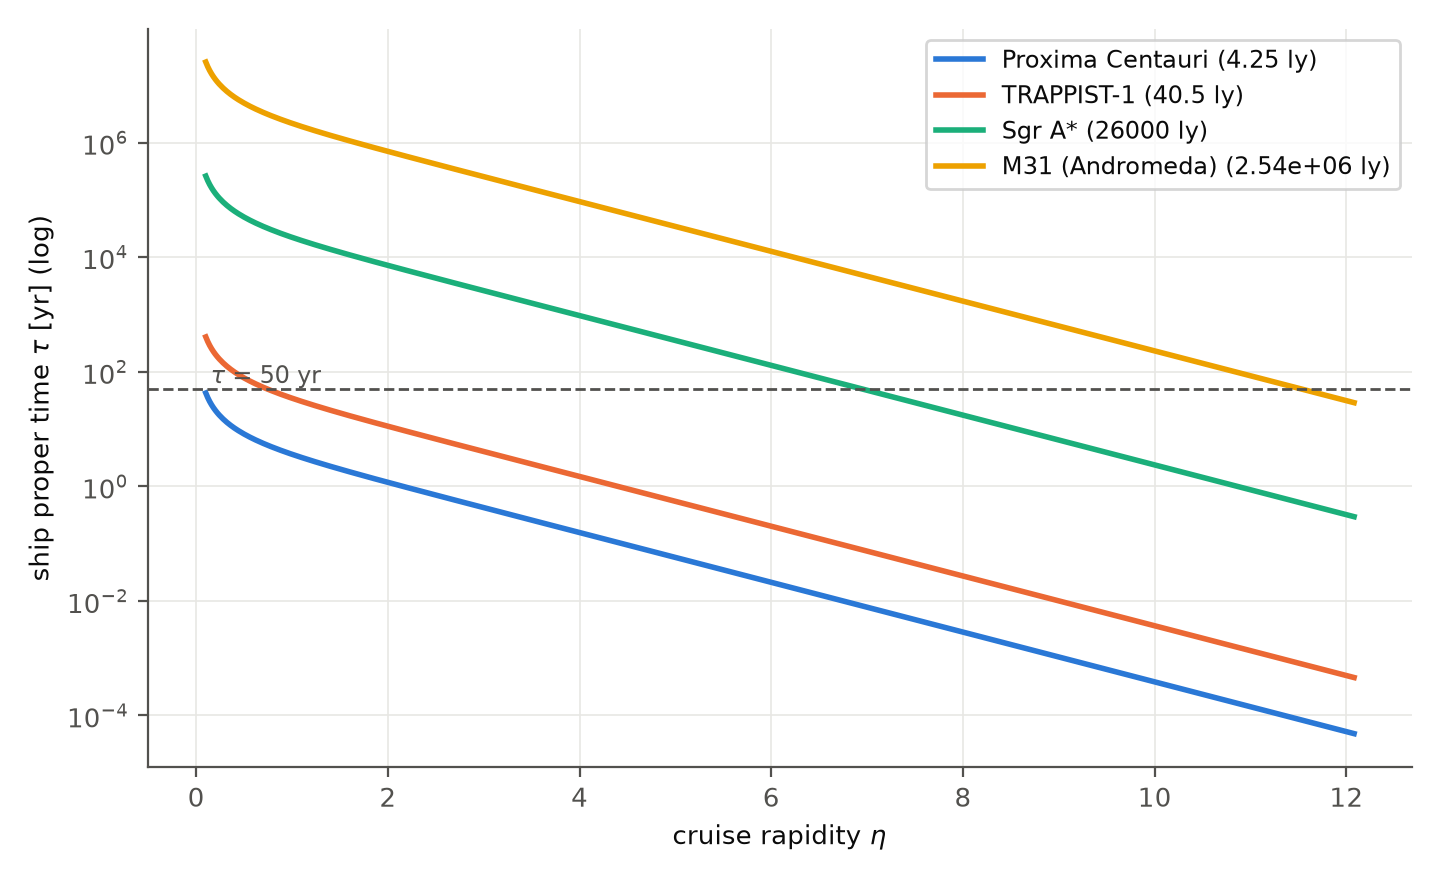
\includegraphics[width=0.82\linewidth]{figures/fig1_contour.png}
\caption{四つのカタログ行き先への到着ミッションにおける、巡航ラピディティに
対する船内固有時間。50 年等高線を併記する。交点は表~\ref{tab:contour}の
$\eta_{50}$ に対応する。}
\label{fig:contour}
\end{figure}

\subsection{三層時間最適プロファイルと拘束レジーム交差}

固定 $\Delta\eta$ の時間最適機動はフロンティアをほとんど至るところで飽和
させる(文献~\cite{le-steering}の定理8)から、最小時間は動く壁に沿う求積
$T = R\int_0^{\Delta\eta} d\eta'/\lambda_{\rm tier}(x_0 e^{-3\eta'})$ で
与えられる。シェルは放射し、$x$ は下がり、壁はバーン中に広がる。この騎乗
時間を三層すべてで評価する(図~\ref{fig:bracket}、表~\ref{tab:bracket})。
実効 [N] 帯は $x_0 = 0.3$ に対し $\eta_{\rm fb} = \ln(x_0/0.1)/3 = \NmEtaFb$
でサンプル域を出て厳密天井へフォールバックし、フォールバック点はすべての
プロファイルに記録される。$\Delta\eta \gtrsim 1$ では実効と天井の時間が収束
し、括りは自動的に締まる。床 tier は桁違いに遅く $e^{3\Delta\eta}$ で増大
するが、これは証明の保守性であって自然の性質ではなく、SI 単位では
$R = 1$ km の床 tier バーンでさえ $\Delta\eta = 0.24$ でミリ秒である。

三層はまた、拘束構成の構造的事実を特定する(図~\ref{fig:tiers})。薄殻
フロンティアスキャン $\underline{g}(x)$ [N] は厚壁天井 $(4/5 - x)/2$ [R] と
$x^* \approx \NmXstar$($\lambda^* \approx \NmLamstar$、公表ピンの線形補間の
下)で交差する。$x^*$ の下では優勢エネルギーのフロンティアが束縛し、上では
厚壁実現可能性が束縛する。$x^*$ を超える薄殻カタログ値は分布的理想化での
み到達可能である。我々の知る限り、第\ref{sec:intro}節に述べた系統的検索の
範囲で、この交差はこれまで定量化されていない。物理的内容は原論文自身の
許容性窓の入れ子と整合的であり、交差は操作レジームの切り替えを定量化した
ものである。

\begin{table}[t]
\centering
\caption{$x_0 = 0.3$ でのフロンティア騎乗最小時間($R$ 単位。SI へは
$R/c$ を乗じる)。天井列は到達不能な下限であり(天井は開条件)、
フォールバック列は [N] 帯がサンプル域を出る点を示す。}
\label{tab:bracket}
% AUTO-GENERATED by scripts/make_paper_numbers.py — DO NOT EDIT
\begin{tabular}{rrrrr}
\hline
$\Delta\eta$ & $T_{\rm floor}/R$ & $T_{\rm eff}/R$ & $T_{\rm ceil}/R$ & $\eta_{\rm fb}$ \\
\hline
0.1 & 1e+03 & 0.515 & 0.37 & -- \\
0.24 & 2.58e+03 & 1.22 & 0.824 & -- \\
0.5 & 6.88e+03 & 2.25 & 1.57 & 0.366 \\
1 & 3.01e+04 & 3.56 & 2.88 & 0.366 \\
2 & 5.65e+05 & 6.08 & 5.39 & 0.366 \\
3 & 1.12e+07 & 8.58 & 7.89 & 0.366 \\
5 & 4.53e+09 & 13.6 & 12.9 & 0.366 \\
8 & 3.67e+13 & 21.1 & 20.4 & 0.366 \\
12 & 5.98e+18 & 31.1 & 30.4 & 0.366 \\
\hline
\end{tabular}

\end{table}

\begin{figure}[t]
\centering
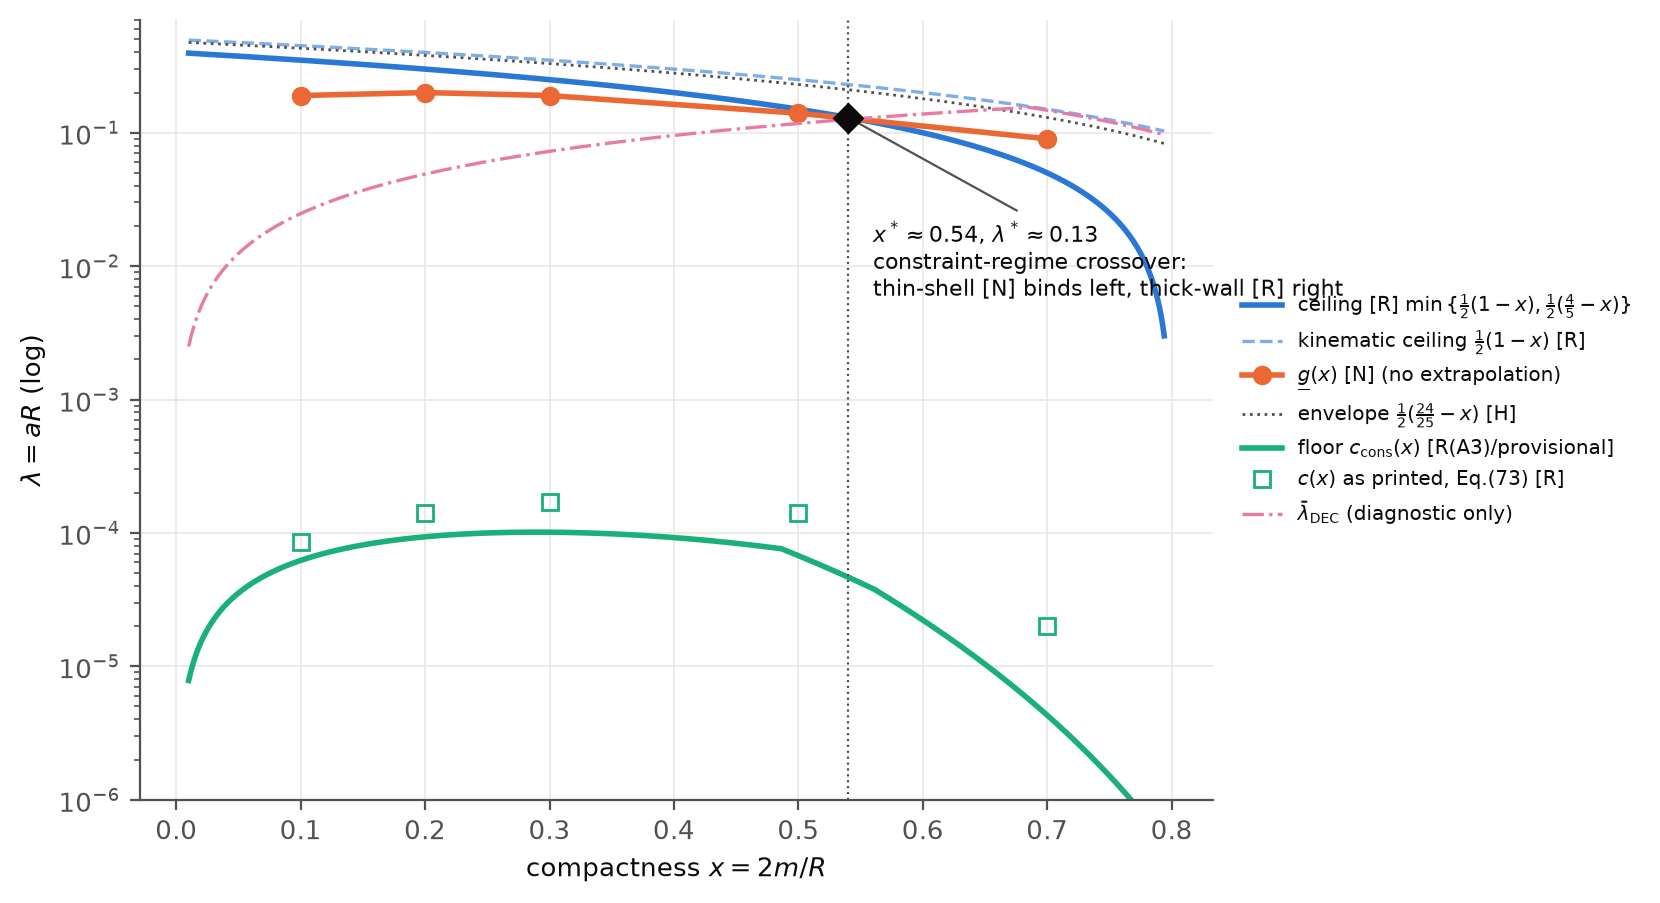
\includegraphics[width=0.95\linewidth]{figures/fig2_tiers.png}
\caption{$\lambda = aR$ に対する三層拘束系。式(73)の印字床値(白抜き
四角)、我々の保守床(実線)、実効帯(丸)、天井、発見法的包絡線 [H]、
凍結形状診断(一点鎖線、拘束には不使用)。菱形は拘束レジーム交差
$x^* \approx \NmXstar$ を示す。}
\label{fig:tiers}
\end{figure}

\begin{figure}[t]
\centering
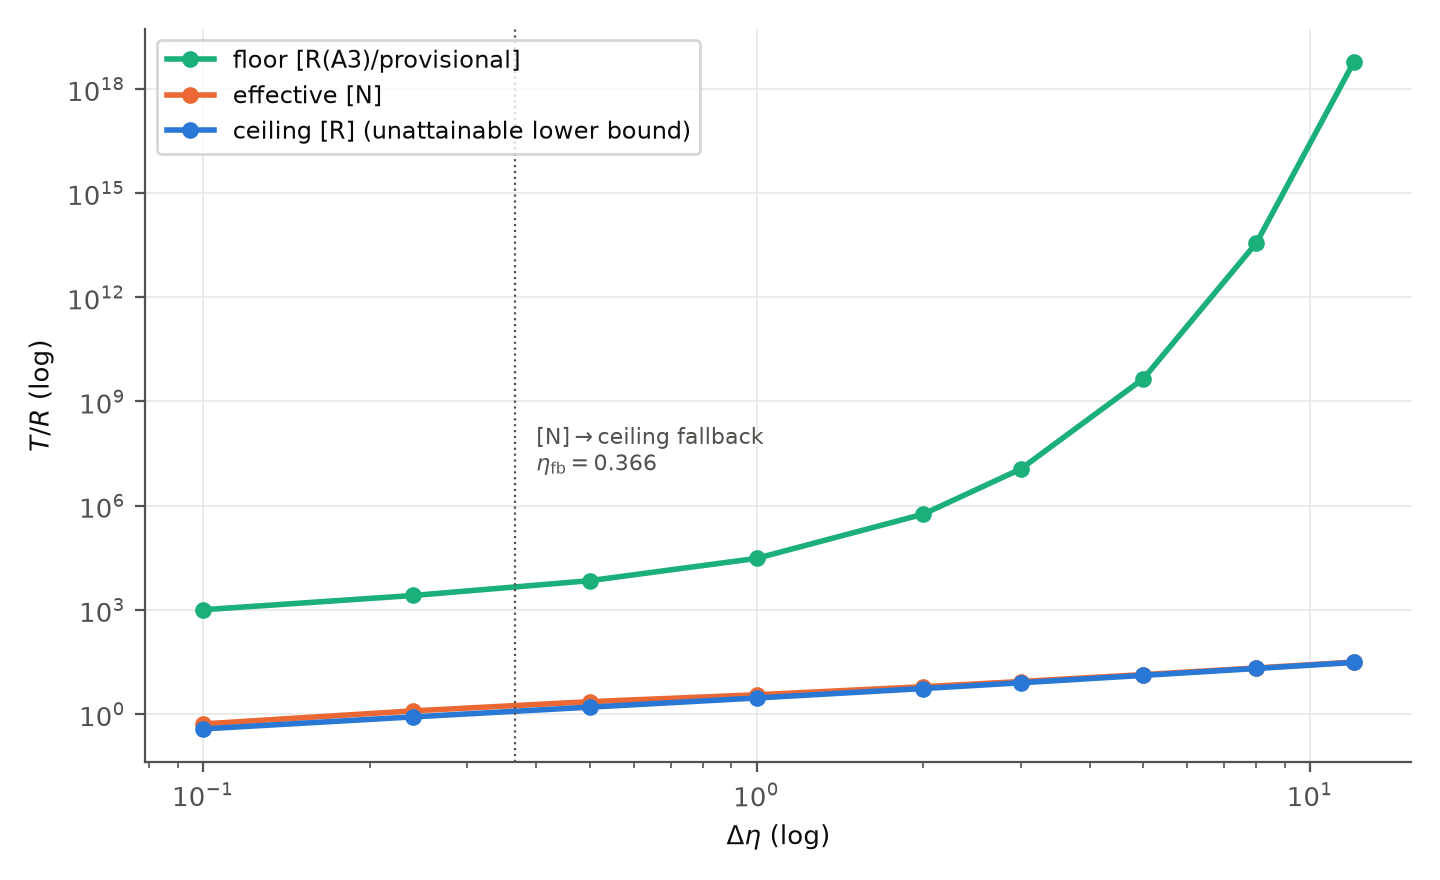
\includegraphics[width=0.8\linewidth]{figures/fig3_bracket.png}
\caption{$x_0 = 0.3$ における三層の最小騎乗時間対 $\Delta\eta$。実効と天井は
フォールバック点を超えると収束し、床は $e^{3\Delta\eta}$ で増大する。}
\label{fig:bracket}
\end{figure}

\subsection{SI レイヤー}

無次元カタログは単一の認証済みモジュールを通じて SI に変換される。
$x_0 = 0.3$、$R = 1$ km でシェル質量は $\NmMassKgKm$ kg $=
\NmMassMsunKm\,M_\odot$、飽和騎乗光度は $L = \tfrac32 x\lambda\,(c^5/G) =
\NmLpeakW$ W $= \NmLpeakLsun\,L_\odot$($R$ に依存しない)、ラピディティ
1 単位のバーンはシェル時間で $\NmBurnMuS\,\mu$s である
(表~\ref{tab:si})。惑星質量から恒星質量の物体が、一度にマイクロ秒だけ、
どの超新星よりも明るく燃える。この光度は保存則が操舵に課す対価であり、
正の放射として支払われる。

\begin{table}[t]
\centering
\caption{$x_0 = 0.3$ での SI 換算(質量は $R$ に比例し、ピーク光度
$\tfrac32 x \lambda\,(c^5/G)$ は $R$ に依存しない)。}
\label{tab:si}
% AUTO-GENERATED by scripts/make_paper_numbers.py — DO NOT EDIT
\begin{tabular}{rrrrr}
\hline
$R$ [m] & $m$ [kg] & $m$ [$M_\odot$] & $L_{\rm peak}$ [W] & [$L_\odot$] \\
\hline
100 & 2.02e+28 & 0.0102 & 3.10e+51 & 8.10e+24 \\
1000 & 2.02e+29 & 0.102 & 3.10e+51 & 8.10e+24 \\
10000 & 2.02e+30 & 1.02 & 3.10e+51 & 8.10e+24 \\
\hline
\end{tabular}

\end{table}

\subsection{観測署名: 前方ヌルと減速フラッシュ}

すべての機動プロファイルは、厳密な静止系パターンと特殊相対論的な光行差、
Doppler 増幅、遅延時間圧縮を通じ、F\"uzfa~\cite{fuzfa2019}の機構を再利用して
観測者系光度曲線に写される。三つの事実がカタログを組織する
(図~\ref{fig:fingerprint}--\ref{fig:flash})。

第一に、飽和制御則で加速するシェルは前方極で厳密に暗い。$4\pi n^2 =
3ma(1 - \cos\vartheta)$ は $\vartheta = 0$ で消え、光行差は極を固定し、
我々の認証はこのヌルを厳密有理算術で検証する。接近するシェルはブースト
全期間、正面からは見えない。

第二に、減速はローブを反転する。目的地の観測者は排気を正面から受け、
$\delta^4 = e^{4\eta}$ で増幅され $dt_{\rm obs}/du = e^{-\eta}$ で到着時間
圧縮される。飽和減速脚に沿って受信フラックスは閉形式の減衰則
$F \propto e^{7\eta - 3\Delta\eta_{\rm tot}}$ に従う。これは増幅と
Tsiolkovsky 質量履歴の合成で得られ、M31 到着($\Delta\eta_{\rm tot} = 24$)
では $e^{7\eta - \NmFlashExp}$、ピーク $F D^2$ は幾何単位で $\NmFlashPeak$
(カタログ値は閉形式と $10^{-12}$ より良く一致)、減衰スケールは
$e^{-\eta}/(7\lambda) \approx \NmFlashDecay\,R$、$R = 1$ km で約
$\NmFlashPs$ ps である。低ラピディティの到着はマイクロ秒に伸びる。到着型
ミッションはしたがって対をなす。$t \approx 0$ の出発側バーストと、経路の
光渡り一回分あとの目的地側フラッシュである。

第三に、二つの層を縫うエネルギー閉合は厳密である。すべてのプロファイルの
光度曲線の積分は $m_0 - m_f$ と $10^{-10}$ で一致し(認証 C15)、時刻表と
光度曲線は同じ積分の二つの読みである。

\begin{figure}[t]
\centering
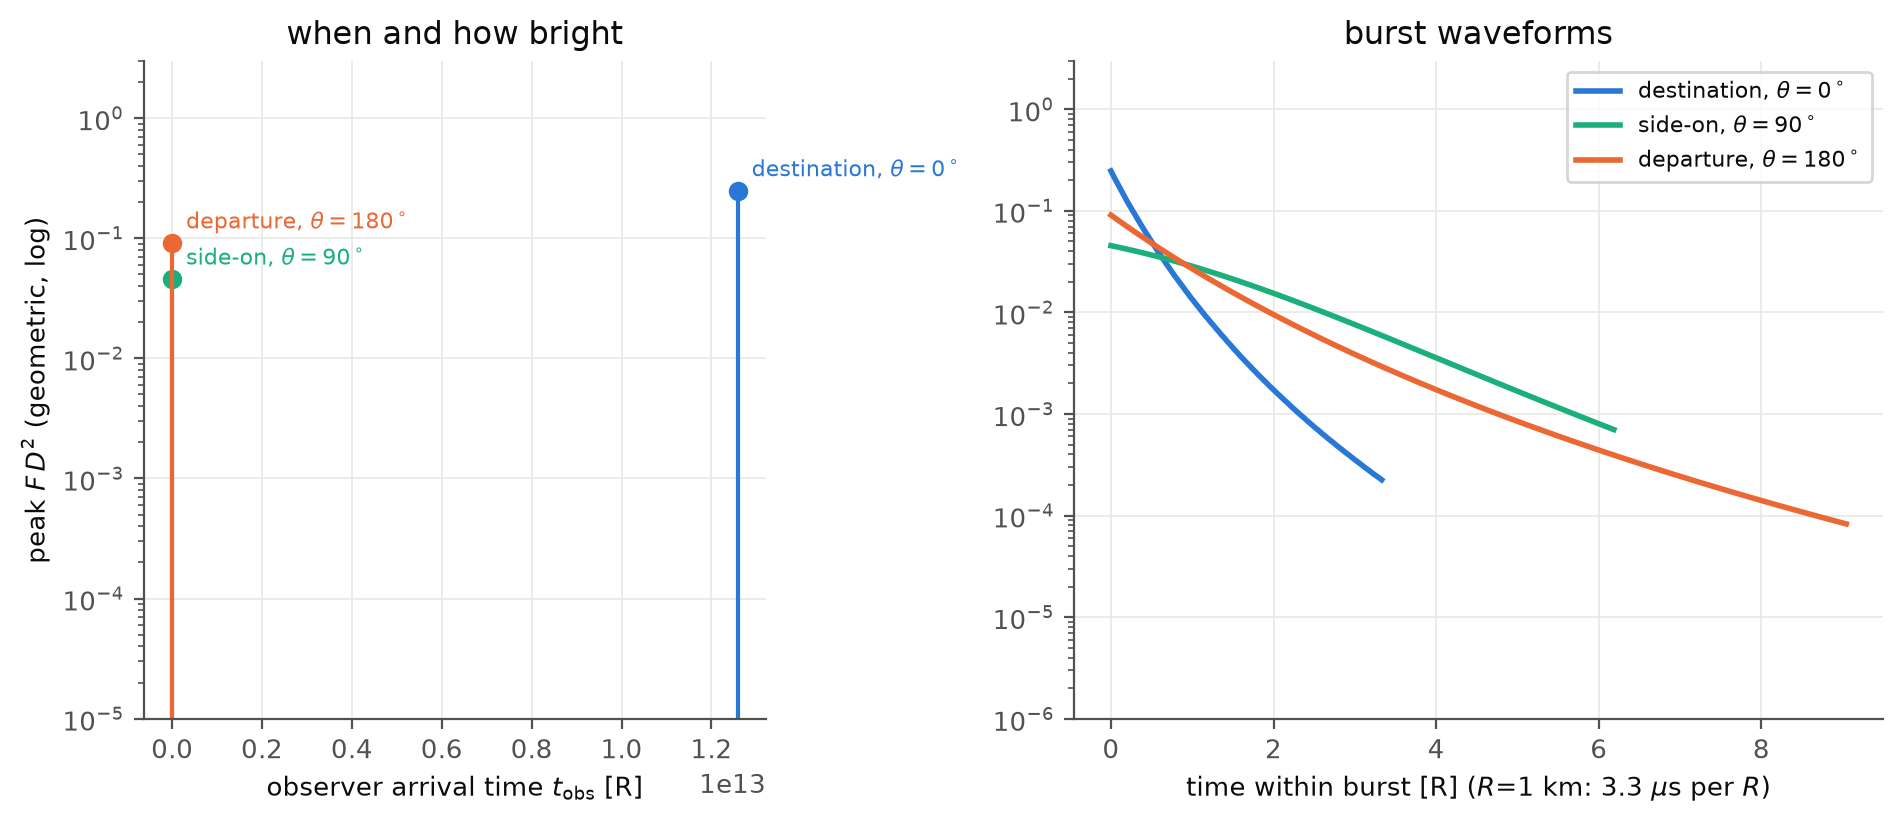
\includegraphics[width=\linewidth]{figures/fig4_fingerprint.png}
\caption{到着ミッションの指紋(プロキシマ、$\eta = 1$)。左は三つの標準
観測者が見る過渡の到着スケジュール、右はバースト波形である。目的地の
フラッシュが最も明るく最も短い。}
\label{fig:fingerprint}
\end{figure}

\begin{figure}[t]
\centering
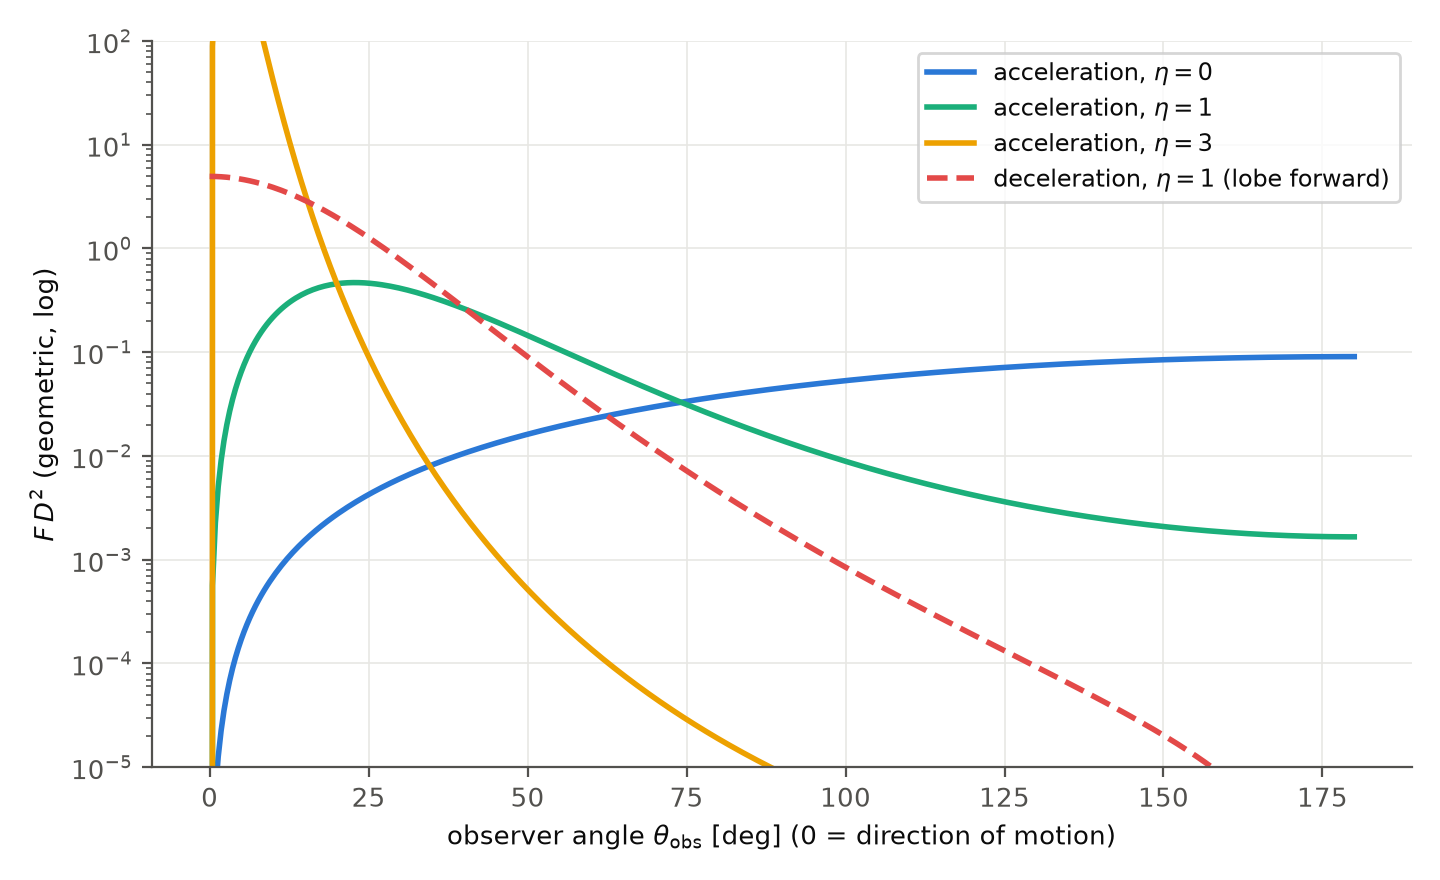
\includegraphics[width=0.8\linewidth]{figures/fig5_pattern.png}
\caption{数個のラピディティにおける飽和バーンの観測者系角度パターンと、
減速バーンの反転ローブ。加速パターンの前方ヌルは厳密である。}
\label{fig:pattern}
\end{figure}

\begin{figure}[t]
\centering
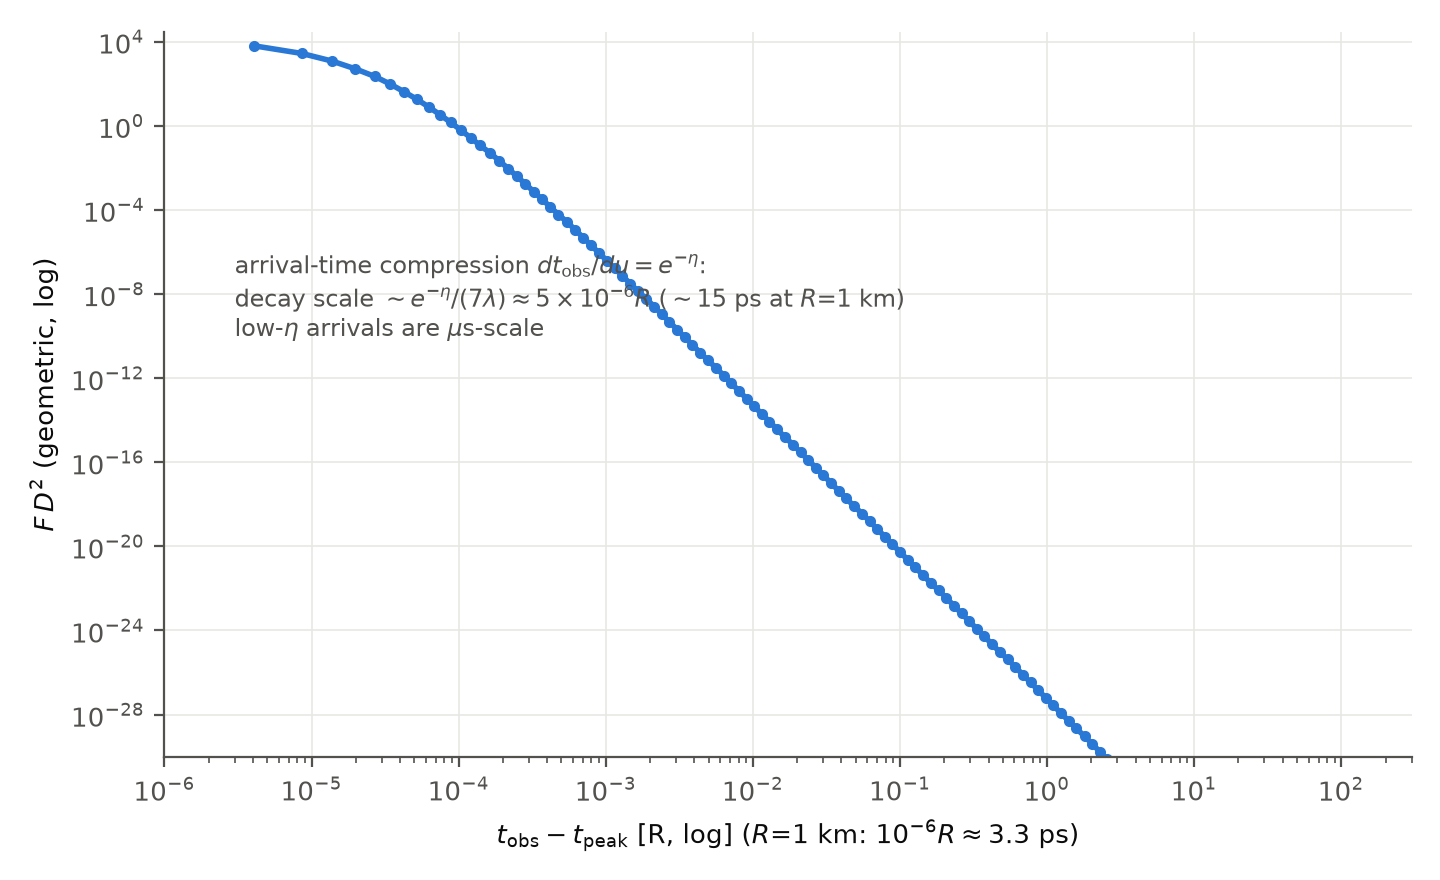
\includegraphics[width=0.8\linewidth]{figures/fig6_flash.png}
\caption{目的地から見た M31 減速フラッシュ(ピークからの対数時間)。到着
時間圧縮が $63R$ の長さのバーンをピコ秒級の過渡に変える。}
\label{fig:flash}
\end{figure}

\subsection{重力波静寂判別子}

最小放射機動は Damour 双極子であり、その上で外部は重力波を放射しない。
スピン上げ演算子が $\ell \leq 1$ の放射を消すため Bondi news は恒等的に
消える。この性質は光子ロケットについて Damour~\cite{damour}が確立し、
文献~\cite{le-steering}の news 静寂類で厳密に成り立つ。純双極子からの逸脱は
放射する。news エネルギーは $\ell \geq 2$ 漏洩振幅の正定値二次形式であり、
重力波出力は二次で増える一方、コリメーション強化による燃料節約は一次で
しか増えない。したがってモデルは反証可能な連合予言、すなわち同位置・
同時刻で重力波対応天体を持たない測光過渡を与え、同じ二チャネルは機動自体の
純度計としても働く。ワープドライブ崩壊との対比は鋭い。Alcubierre 級バブルの
封じ込め失敗は重力波バーストを一次信号として放射する~\cite{clough}。判別
平面の正反対の隅である。正エネルギーワープバブルからの放射探索の
提案~\cite{lentzfelton}は、必要な波形と角度パターンを本カタログから直接
引くことができる。

\section{議論}\label{sec:discussion}

\subsection{限界}

カタログの妥当性境界はラベルが担う。加速厚壁のエネルギー条件定理は原理論で
未解決であり(著者自身が future work として明記している)、厚壁実現可能性は
後方極実効コンパクト度への静的窓として課される。実効帯 $\underline{g}(x)$
は $x \in [0.1, 0.7]$ でのみ定義され、外挿されない。騎乗プロファイルは域外で
厳密天井にフォールバックし、フォールバック点が記録される。署名は
ボロメトリックであり、パラメータ化シナリオのみを伴う($R = 1$ km のシェルを
黒体と読めば硬ガンマ域にピークするが、これはラベル付きの仮定であり排気の
微視物理の主張ではない)。床 tier は第\ref{sec:methods}節に記した照合が
終わるまで暫定である。本研究が導入した解釈上の仮定(実働バーンの無次元
閉包、ミッションバーン規約、床鎖の読み、薄殻クランプの根拠)はデータ公開物
の仮定台帳に列挙されている。

\subsection{時間・光度平面での位置}

予言される過渡は、既知の天体物理クラスが占めない時間・光度平面の隅を
占める。マイクロ秒からピコ秒の持続、超新星ピークをはるかに超える等方等価
光度、単発または対のイベント、到着前の厳密な前方ヌル、全期間の重力波
静寂である。いかなる装置での検出可能性についても述べない。物理的な幾何
(ビーム幅 $\sim e^{-\eta}$、非反復、経路の光渡り一回分をまたぐ対)だけで、
スケーリング則の水準で、反復する現象や重力波的に大きな現象からこのクラスを
区別するに足りる。

\subsection{床値の再現性}

未解決の検証項目を一つ、招待として再掲する。式(73)の印字された床評価値は、
論文にも固定コミットの公開コードにも閉形式が現れない三つの上限量を要する。
我々の保守的再構成は文書化された読みの下でそれらを上から抑え、印字値の
厳密に下に落ちる。式(73)の背後の計算が公開されれば、このギャップは閉じ、
本カタログの床 tier はおそらく鋭くなる。

\section{データ公開}\label{sec:data}

全パイプライン(認証済みライブラリ、認証スイート C1--C19、カタログ、署名
ファイル、図表生成器、数値マニフェスト、仮定台帳)は [GitHub URL、Zenodo
DOI はリリース時発行] で公開し、プロジェクトリポジトリの [リリース時注入の
コミットハッシュ] に固定する。検証スイートは 1 分未満で走り、本論文の
すべての数値を再現する。

\section*{謝辞}

本研究は An T. Le による warpax~\cite{warpax-code} と world\_tube 再現
コード~\cite{worldtube}(いずれも MIT ライセンス)を使用した。すべての計算、
実装、起草は第\ref{sec:methods}節に記した人間ゲート付きプロトコルの下で
Claude(Fable 5, Anthropic)が行った。人間著者はプロジェクトを指揮し、
すべての決定ゲートを裁定し、内容に責任を負う。

\begin{thebibliography}{99}
\bibitem{le-steering} A. T. Le, ``Steering a warp drive without exotic
matter,'' arXiv:2606.22531 (2026).
\bibitem{le-boundary} A. T. Le, ``On the boundary cost of source-consistent
warp shells,'' arXiv:2605.25417 (2026).
\bibitem{le-warpax} A. T. Le, ``Observer-robust energy condition
verification for warp drive spacetimes,'' arXiv:2602.18023 (2026).
\bibitem{alcubierre} M. Alcubierre, Class. Quantum Grav. \textbf{11}, L73
(1994).
\bibitem{ssv} J. Santiago, S. Schuster, and M. Visser, Phys. Rev. D
\textbf{105}, 064038 (2022).
\bibitem{pfenning} M. J. Pfenning and L. H. Ford, Class. Quantum Grav.
\textbf{14}, 1743 (1997).
\bibitem{lobo} F. S. N. Lobo and M. Visser, Class. Quantum Grav.
\textbf{21}, 5871 (2004).
\bibitem{lentz} E. W. Lentz, Class. Quantum Grav. \textbf{38}, 075015
(2021).
\bibitem{celmaster} B. Celmaster and S. Rubin, arXiv:2511.18251 (2025).
\bibitem{bobrick} A. Bobrick and G. Martire, Class. Quantum Grav.
\textbf{38}, 105009 (2021).
\bibitem{fuchs} J. Fuchs, C. Helmerich, A. Bobrick, L. Sellers,
B. Melcher, and G. Martire, Class. Quantum Grav. \textbf{41}, 095013
(2024).
\bibitem{helmerich} C. Helmerich, J. Fuchs, A. Bobrick, L. Sellers,
B. Melcher, and G. Martire, Class. Quantum Grav. \textbf{41}, 095009
(2024).
\bibitem{fuzfa2019} A. F\"uzfa, Phys. Rev. D \textbf{99}, 104081 (2019).
\bibitem{fuzfa2020} A. F\"uzfa, W. Dhelonga-Biarufu, and O. Welcomme,
Phys. Rev. Research \textbf{2}, 043186 (2020).
\bibitem{kinnersley} W. Kinnersley, Phys. Rev. \textbf{186}, 1335 (1969).
\bibitem{damour} T. Damour, Class. Quantum Grav. \textbf{12}, 725 (1995),
arXiv:gr-qc/9412063.
\bibitem{bonnor} W. B. Bonnor, Class. Quantum Grav. \textbf{11}, 2007
(1994).
\bibitem{vdgk} U. von der G\"onna and D. Kramer, Class. Quantum Grav.
\textbf{15}, 215 (1998).
\bibitem{israel} W. Israel, Nuovo Cimento B \textbf{44}, 1 (1966).
\bibitem{clough} K. Clough, T. Dietrich, and S. Khan, Open J. Astrophys.
\textbf{7} (2024), arXiv:2406.02466.
\bibitem{lentzfelton} E. W. Lentz and R. C. Felton, arXiv:2405.19381
(2024).
\bibitem{worldtube} A. T. Le, world\_tube reproduction code,
\url{https://github.com/anindex/world_tube} (MIT license).
\bibitem{warpax-code} A. T. Le, warpax v1.3.0,
\url{https://github.com/anindex/warpax} (MIT license).
\end{thebibliography}

\end{document}
